\clearpage
\section{The Experiment}

\subsection{The Large Hadron Collider\label{sec:lhc}}

The Large Hadron Collider (LHC) is a particle accelerator and collider
housed 100 meters undeground in a 27 km long circular tunnel situated 
beneath the Swiss-French border. The collider consists of two 
counter-circulating particle beams which are made to collide at four points 
along the ring. Figure~\ref{fig:lhc} shows the location of the LHC and 
the four main detectors each housed at a different collision point.\\
\indent The machine contains four straight long sections where acceleration, 
collimation, and beam dump systems are housed. The longer arc sections are
in fact comprised of 1232 straight dipole magnets 15 meters in length designed to contain 
the particle beams in a circular path. Each section is held at a 
super-conductive temperature of 2 Kelvin which provides magnetic fields up to 8
Tesla that steer the beams. Higher order multi-pole magnets are 
placed near the interaction points to collimate and align the 
colliding beams. Unwanted beam interaction with residual gas in the beam pipes
is minimized by vacuuming the beam pipes to pressures below $10^{-10}$~mbar.

\begin{figure}[h!]
  \begin{center}
      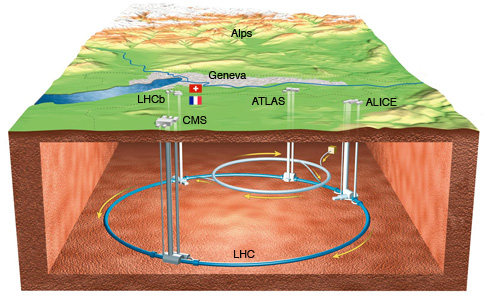
\includegraphics[width=0.40\textwidth,]{figures/CERNMap.jpg}
      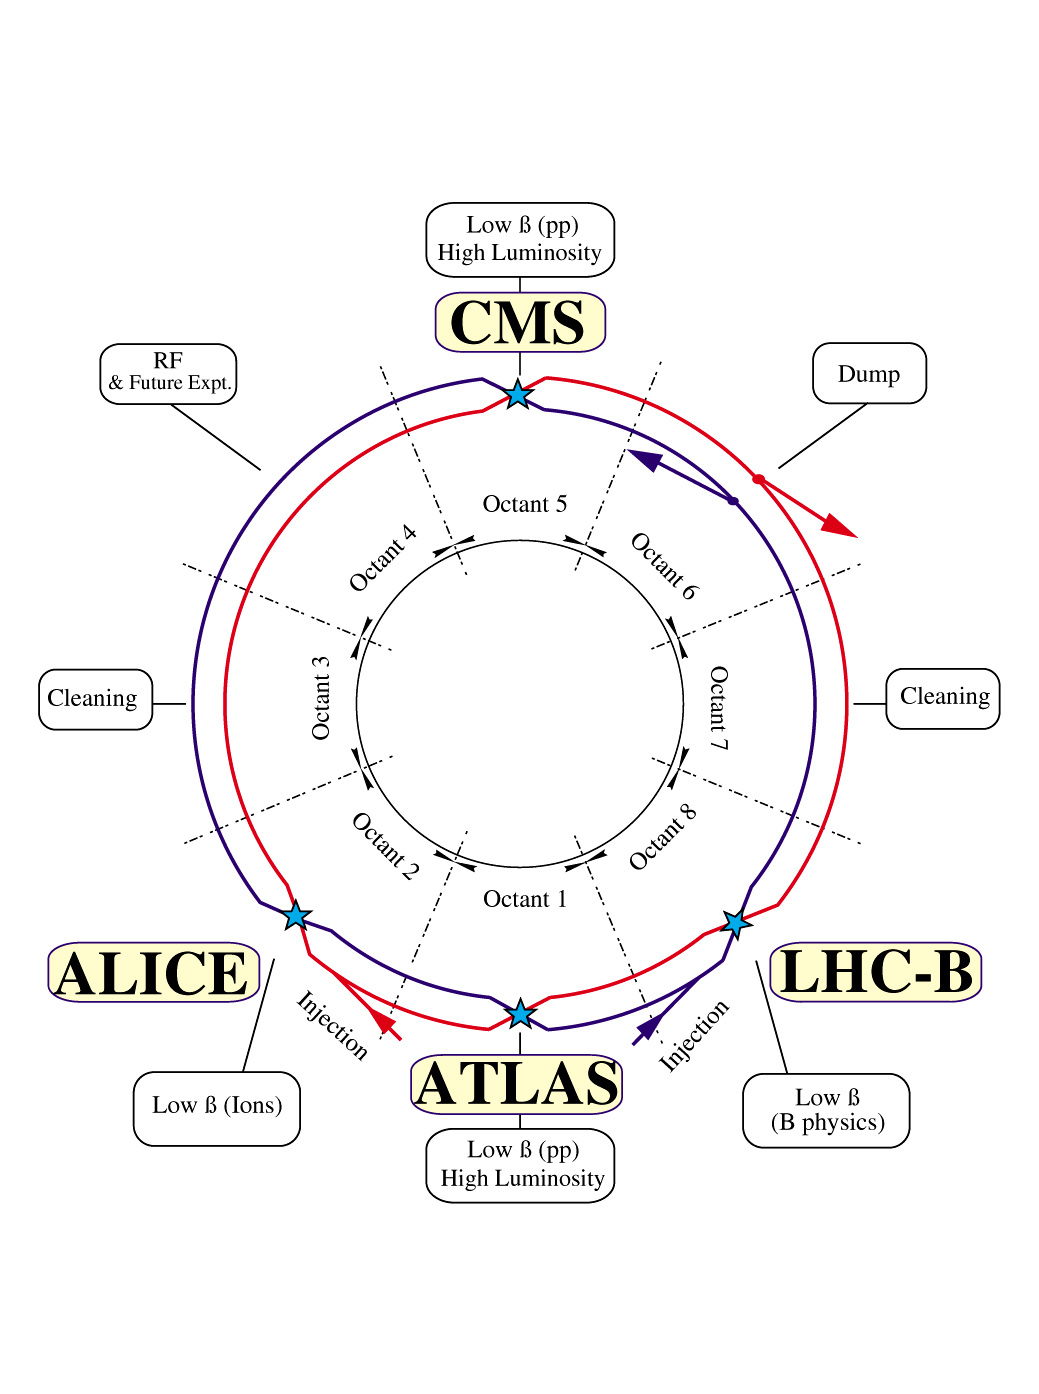
\includegraphics[width=0.35\textwidth,]{figures/lhc-pho-1997-060.jpg}
      \caption{\label{fig:lhc} Left: a geographical map of the location of the LHC. Right: 
      the layout of LHC.}
  \end{center}
\end{figure}

\indent The protons are accelerated along straight sections of the ring where 
Radio-Frequency (RF) cavities generating electromagnetic fields are 
tuned to deliver protons a ‘kick’ of energy at each revolution in the accelerator ring. 
Protons that are ideally timed and have exactly the desired energy, will feel 
a zero accelerating force from the RF cavity, while protons with slightly different 
energies that arrive earlier or later are decelerated or accelerated. As a result, 
the proton beams are divided in discrete ``bunches'' of protons. Each bunch, before collision,
measures $16~\micron$ transversally and $\sim\!\!30$~cm long. Bunches are separated 7~m apart.
The LHC has been designed to operate with 2808 bunches per beam, with about $10^{11}$ protons per bunch. 
The figure of merit for colliders such as the LHC is the luminosity, a quantity 
influencing the rate of collisions. The instantaneous luminosity depends on the number of protons
per beam, the transverse dimensions of the beams (the more the beams are squeezed,
the higher the probability that a proton-proton collision takes place), and the bunch-
crossing frequency. The number of events N of a certain process with cross section σ
produced per second can be expressed as
%
\begin{equation}
  \label{eq:lumi}
  \frac{dN}{dt} = \,\mathcal{L} \times \sigma
\end{equation}
%
The luminosity integrated over the course of the three separate proton-proton collision runs
is shown in Figure~\ref{fig:int_lumi}. 
%The large increases in delivered luminosity in such
%a short time indicates both the phenomenal success of LHC commissioning and running, and 
%the challenge presented to CMS to accommodate new running conditions nearly continuously, 
%in particular to design and deploy suitable trigger tables, readout thresholds, 
%reconstruction algorithms, and analysis methods.

\begin{figure}[h!]
  \begin{center}
      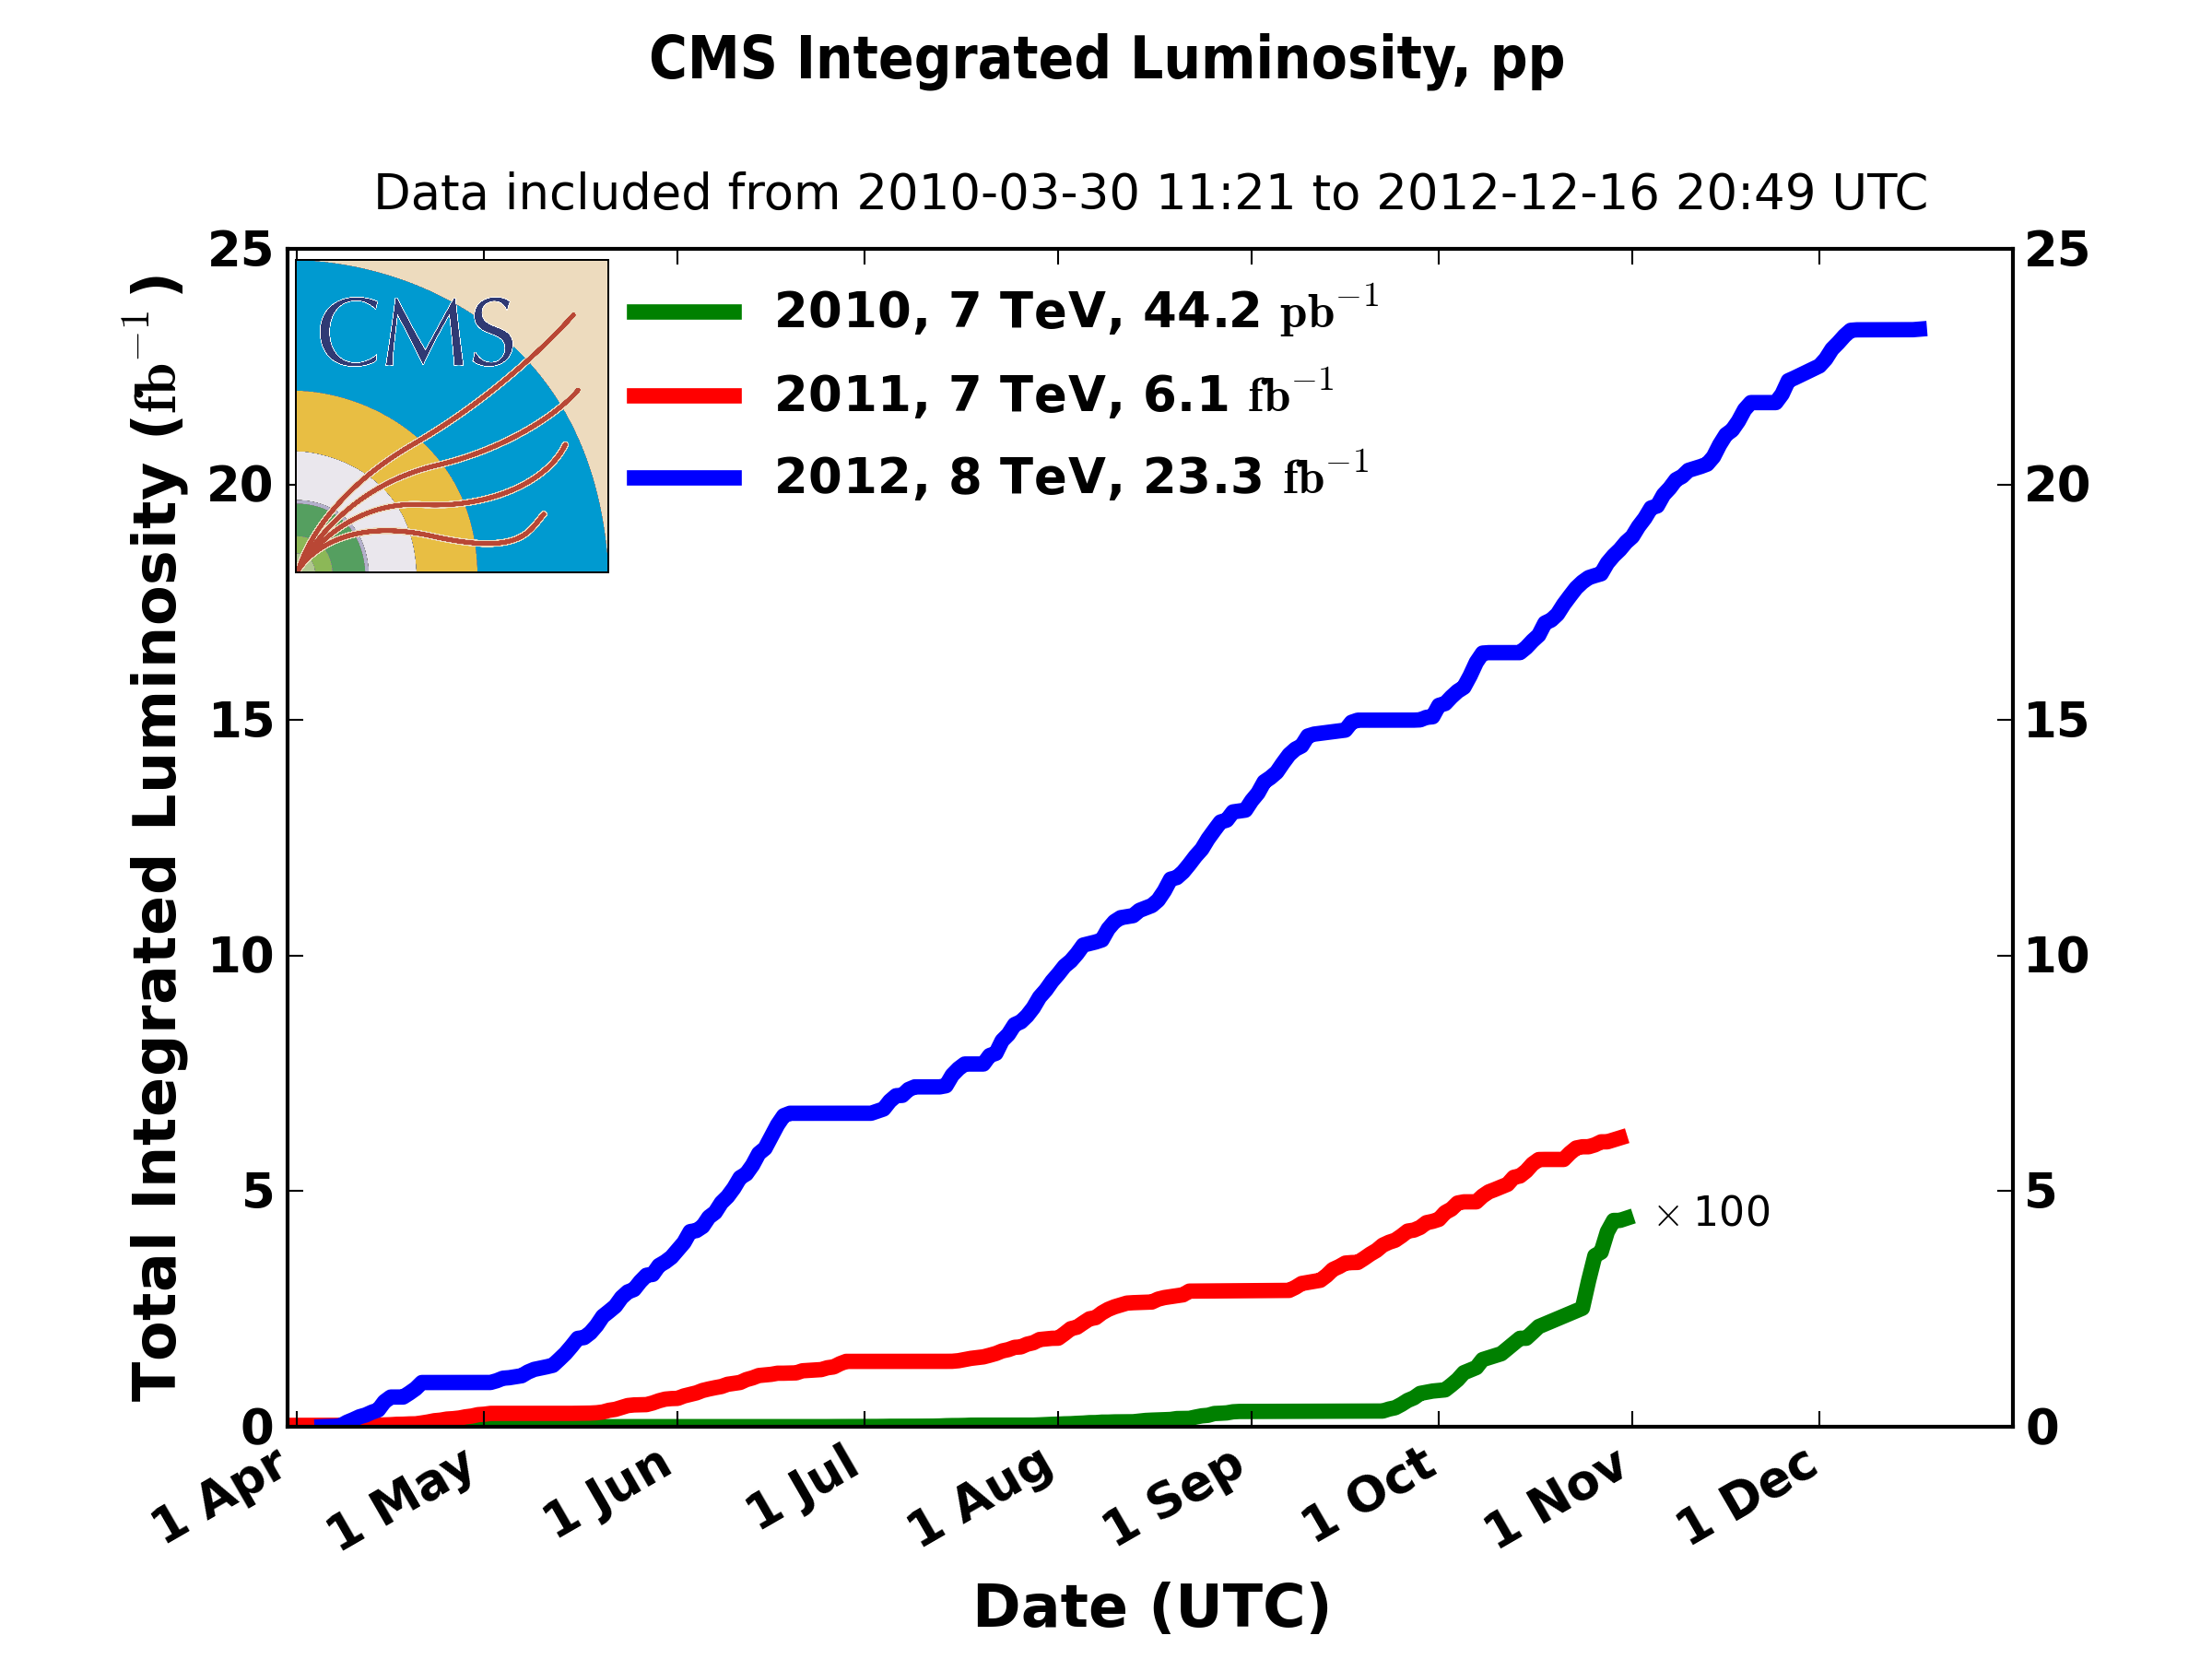
\includegraphics[width=0.40\textwidth,]{figures/int_lumi_cumulative_pp_2.png}
      \caption{\label{fig:int_lumi} The luminosity integrated over the course of the three 
      separate proton-proton collision runs as recorded by CMS.  
      Note: the 2010 curve is multiplied by 100 for legibility.}
  \end{center}
\end{figure}
\subsubsection{High energy proton collisions}
The 
The interactions sought and the SM processes that appear as backgrounds are those in 
which substantial momentum is transferred between the constituent partons of the LHC's 
colliding protons; the incident protons are destroyed and energetic outgoing elementary 
particles and proton remnants are produced. The distributions of what fraction of a 
proton's momentum a constituent gluon or quark carries are given by parton distribution 
functions (PDFs). For a particular production process, e.g. $pp \ra \ttbar$ or 
$pp \ra \bar{g}\bar{g}$, there are various parton scattering processes, e.g. 
from initial gg or $q\bar{q}$, which contribute; their cross sections are integrated over momentum fraction according to 
the PDFs and summed to obtain a total production cross section.
Results of such cross section computations for a variety of processes are shown
in Figure~\ref{fig:crossSec}.

\begin{figure}[h!]
  \begin{center}
      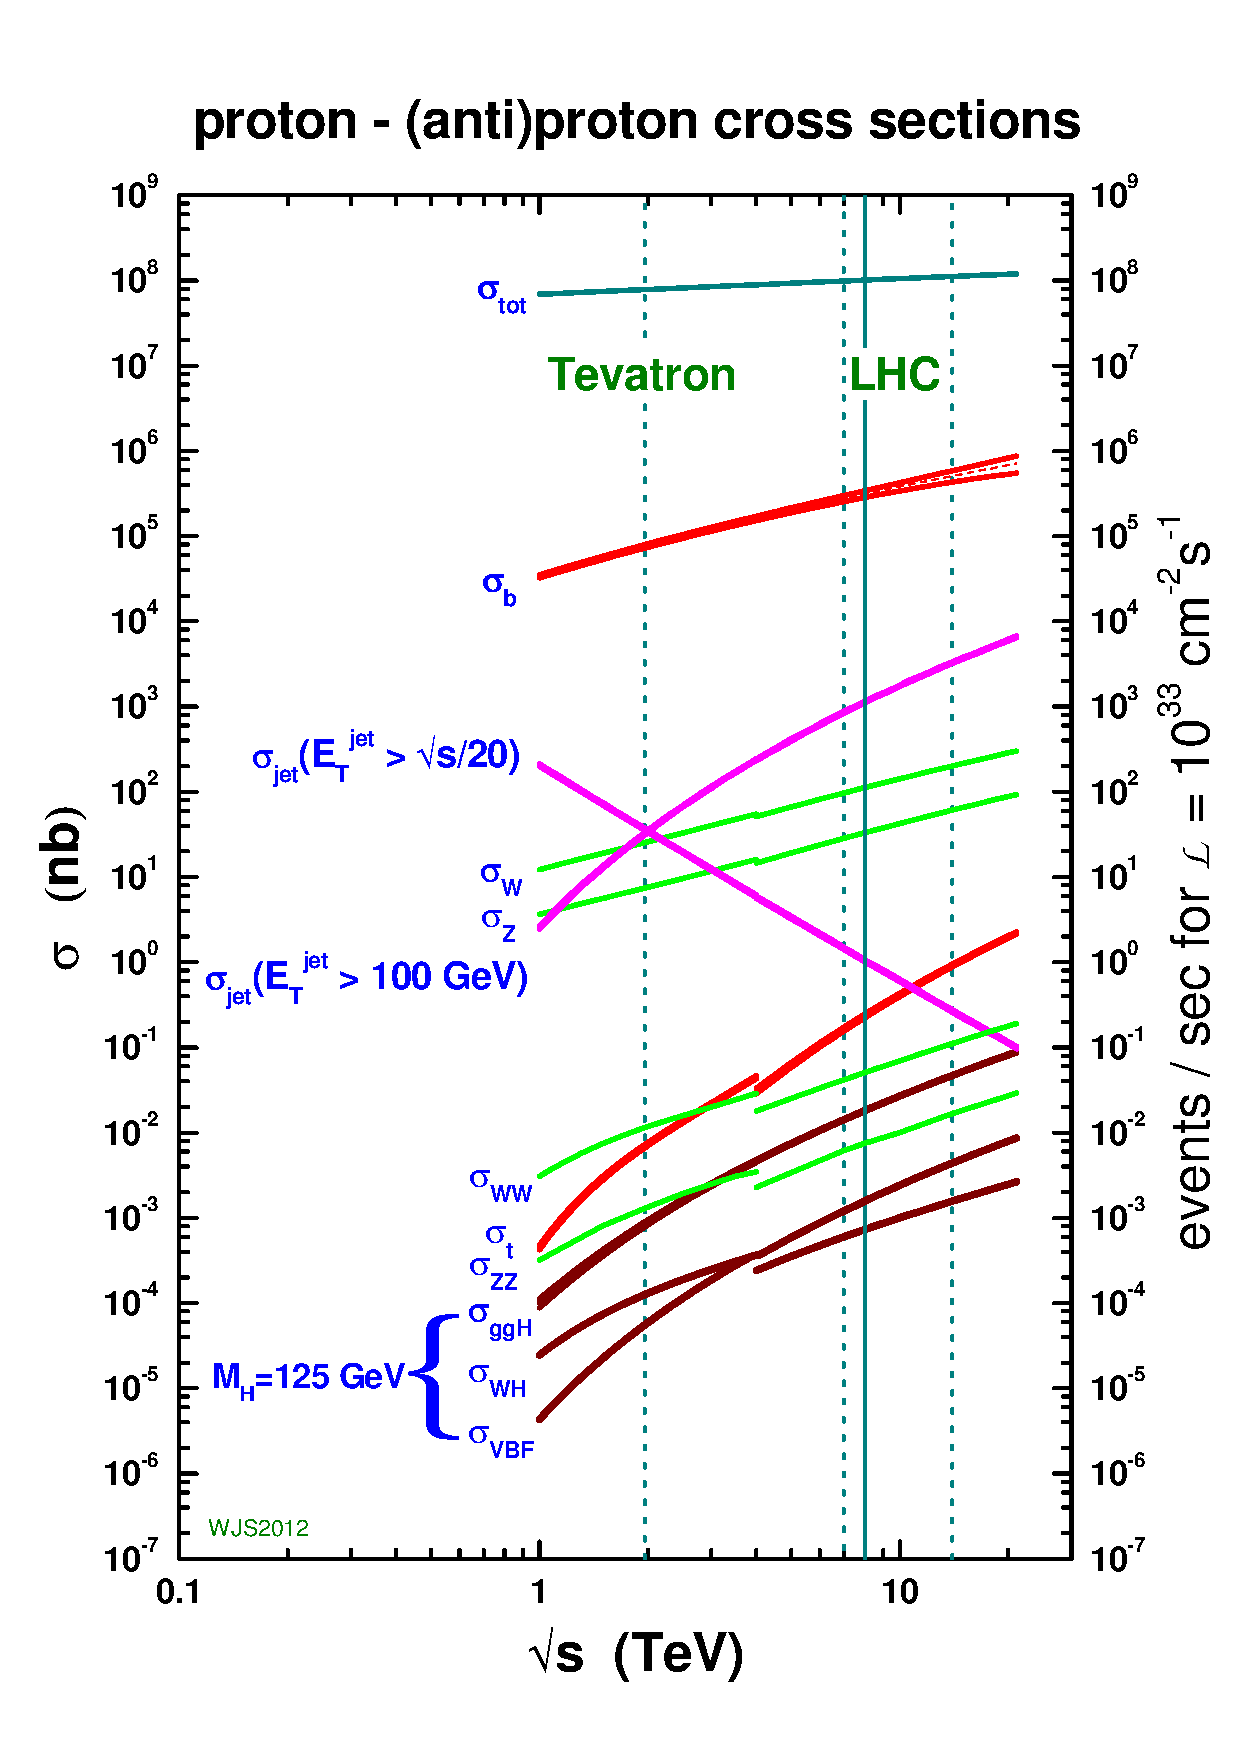
\includegraphics[width=0.40\textwidth,trim=0 2cm 0 0]{figures/crosssections2012_v5}
      %      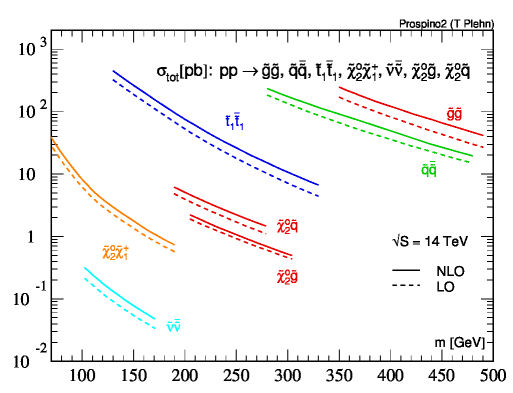
\includegraphics[width=0.40\textwidth,]{figures/PEacs.png}
      \includegraphics[width=0.5\textwidth, ]{figures/nlonll_lhc8_tpformat.eps}
      \caption{\label{fig:crossSec} Left: the cross sections (in nb) of various SM processes vs. center-of-mass
              energy in $pp$ collisions when $\sqrt{s}>1$~\TeV, from Ref.~\cite{stirling-xs}. Right: 
              The cross sections (in pb) of various SUSY processes vs. sparticle for $pp$ collisions
              at $\sqrt{s}=8$~\TeV. From Ref.~\cite{Beenakker:1996ed}.} 
  \end{center}
\end{figure}

The potentially tiny rate of sparticle production compared with that
of known processes presents a challenge for the search. In addition, given the total
inelastic cross section of order 50 mb, the luminosity per colliding pair of bunches
achieved at the LHC is sufficiently high that the expected number of interactions that
occur in the same crossing as an interaction of interest is non-negligible. For the data
used in this search, the mean number of such “pile-up” interactions is approximately
20. Quarks or gluons which emerge from a hard-scattering process fragment and eventually 
group into hadrons before observation in a detector. They are visible as energetic
sprays of hadrons called “jets”, which typically leave tracks in the inner detector
and deposit energy in the calorimeters. The center-of-mass of the scattering system
has a boost along the beam-line which varies event-by-event. It is therefore convenient
to discuss jets (as well as other reconstructed particles) in terms of these quantities:
transverse momentum $\pt$ , which is invariant under such boosts, or similarly transverse
energy $\equiv E \sin\left(\theta\right)$, with $0 \leq \theta \leq \pi$ where $\theta$
is the polar angle from the beam-line; and pseudo-rapidity $\eta \equiv −\ln\left( \tan\left(\theta/2\right)\right)$
, of which differences are (approximately) invariant.

\subsection{The Compact Muon Solenoid detector\label{sec:cms}}
\subsubsection{The detector}
The Compact Muon Solenoid (CMS) detector is designed to provide efficient 
identification and measurement of photons, electrons, muons, taus, and hadronic showers
over wide ranges of transverse momentum and direction, and its nearly 4$\pi$ coverage
in solid angle provides accurate measurement of global transverse momentum imbalance. 
It has sufficient granularity to perform these measurements even when 20+
interactions occur simultaneously in a collision of two bunches of protons, and fast
enough response to do so when the time between beam crossings is 25 ns. Its components 
are resistant to damage from radiation, enabling its use to collect substantial
luminosity, and its modularity allows for long-term maintenance and upgrades. When
closed, CMS is a cylinder of length 22 m, diameter 15 m, and mass 12,500 tons. It
is described in detail elsewhere~\cite{1748-0221-3-08-S08004}.\\
\indent The last name of the detector refers to a superconducting solenoid of radius 3 m
and length 12.5 m, which carries 18 kA to provide a longitudinal magnetic field of
3.8 T. It is operated at 4.5~K. This magnet is surrounded by a central fixed ``ring''
and two movable rings on each side, constituting the ``barrel''; it is flanked on each
side by an ``endcap''. The tracking system and calorimeters reside in the magnet
bore. The layout is shown in the bottom plot of Figure~\ref{fig:cms}. The x-axis is taken to point
radially toward the center of the LHC ring, the y-axis to point against gravity, and
the z-axis to form a right-handed coordinate system.

\begin{figure}[h!]
  \begin{center}
      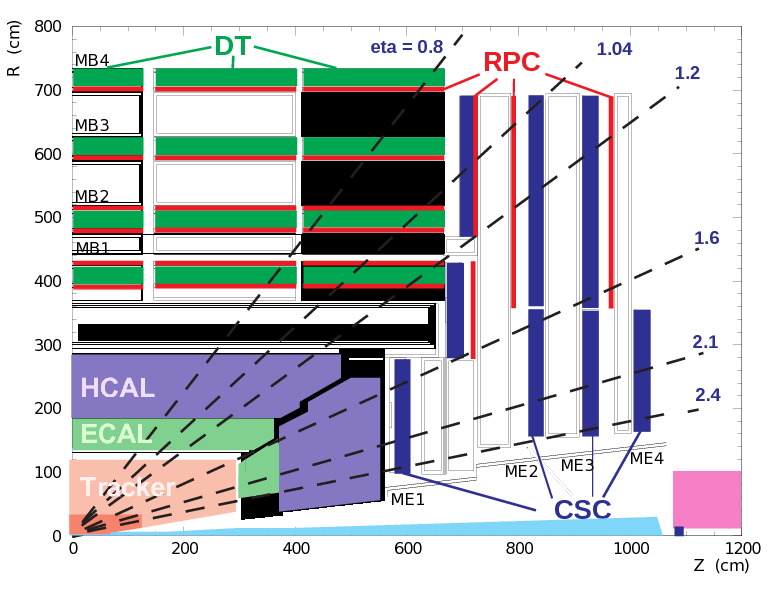
\includegraphics[width=0.65\textwidth, trim = 2cm 0 0 0]{figures/cmsQuad.png}\\
      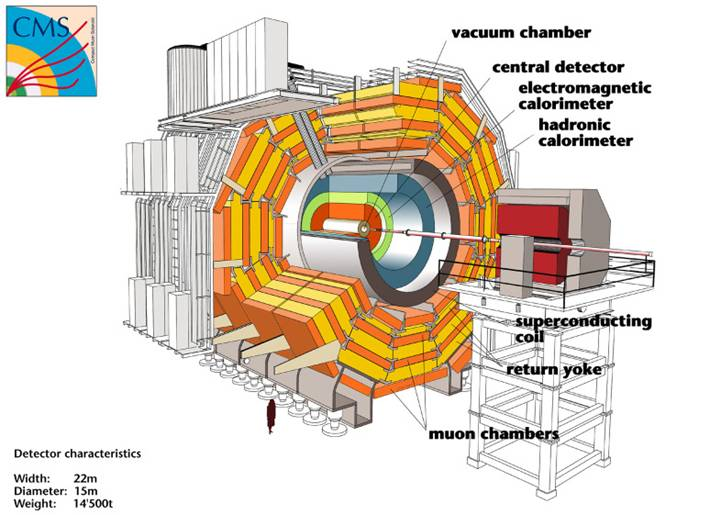
\includegraphics[width=0.65\textwidth,]{figures/CMS_Detector.jpg}
      \caption{\label{fig:cms} Top: a view of one quadrant of CMS. The volume enclosing 
      the tracker is shown in light red, the electromagnetic calorimeter in light green, 
      the hadron calorimeter in lavender, and the forward calorimeter in magenta. 
      The muon detectors are labeled, from Ref.~\cite{2012JInst...7P0002T},
      Bottom: a perspective view of CMS from Ref.~\cite{1748-0221-3-08-S08004}.}
  \end{center}
\end{figure}

The closest subdetector to the beam is the tracker. Charged particles are tracked in 
3 dimensions within a distance of 4.4~cm up to 10~cm from the beam axis with three co-centric layers of hybrid 
pixel detectors totalling 66 million pixels. Two additional layers shaped in disks are placed at each 
end the of the barrel giving the pixel detector coverage up to pseudorapidity $|\eta| < 2.5$.
Leaving the pixel detector, particle continue through 10 barrel layers and 12 endcap disks 
of the silicon strip tracker extending to 1.1~m from the beam axis. The silicon srip tracker
consists of 10 million srips covering a total area $200~\texttt{m}^2$.  This tracking system
provides high transverse-momentum ($\pt$) resolution, efficiency, and primary- and secondary-vertex
resolutions.\\
\indent Surrounding the tracker is the electromagnetic calorimeter (ECAL) consisting of over 60 thousand scintilating 
lead tungstate crystals in the barrel ($|\eta| < 1.48$) and a further 7,500 crystals in each endcap extending
the coverage up to each measuring $|\eta| < 2.5$. The crystals have a front-face cross section
of approximately $22 \times 22~\texttt{mm}^2$ (resp. $28.6 \times 28.6~\texttt{mm}^2$) in the barrel (resp. endcap) with a
length of 23~cm corresponding to $\sim25$ radiation lenghts, i.e. the length which an electron loses
all but $1/e$ of its energy or $7⁄9$ of the mean free path for pair production by a high-energy photons.  
Avalanche photo-diodes detect the scintilated light in the barrel $(|\eta| < 1.479)$ vacuum photo-triodes 
in the endcap $(1.479 < |\eta| < 3.0)$. For extra spatial precision, the ECAL also contains lead-silicon 
sampling detector that sit in front of the endcaps. These allow CMS to distinguish between single high-energy 
photons and close pairs of low-energy photons.\\
\indent The hadron calorimeter (HCAL) consists of alternating layers of brass absorber
and plastic scintillator, which sample hadronic showers, arranged in identical azimuthal units 
into two half-barrels and also into two endcaps. The scintillators are segmented projectively 
into towers of area $\Delta\eta \times \Delta\phi = 0.087 \times 0.087$ for $|\eta| < 1.6$, and 
approximately $0.17 \times 0.17$ for $|\eta| > 1.6$. The light produced in the 
scintillator layers is merged, wavelength-shifted and carried to the photo-cathode 
of a hybrid photo-diode (HPD). The single stage HPD accelerates the liberated electrons 
using a $\sim$7 kV potential difference, which then impinge on a silicon diode. 
The current produced is amplified, digitized, and transmitted via optical links to 
dedicated boards. Coarse data, summed over longitudinal segments (which are present 
for $|\eta| > 1.2$) and time, are transmitted after peak-finding to the calorimeter 
trigger system. The full data, after the suppression of low energy hits to reduce data 
volume, are sent to the data acquisition system (DAQ).\\
\indent Outside of the endcaps are forward 
calorimeters (HF) of steel absorber and quartz fibers, in which relativistic particles 
produce Cherenkov light. They cover the region $3.0 < |\eta| < 5.0$, thereby improving the 
hermeticity of CMS. Their hit-occupancy is histogrammed at 40 MHz to track the delivered
luminosity, and the instantaneous luminosity computed from the histograms is reported each
``luminosity section'', i.e. 218 beam orbits or approximately 23 seconds. The luminosity 
measurement is calibrated by scanning the transverse positions of the beams relative to each 
other to measure their effective overlap~\cite{CMS-PAS-SMP-12-008}.\\ 
\indent The magnet’s flux-return yoke and the endcaps are instrumented with muon detection systems, 
as shown in the top plot of Figure~\ref{fig:cms}. The drift tube (DT), cathode strip chamber 
(CSC), and resistive plate chamber (RPC) systems provide
efficient detection of muons with pseudo-rapidity $|\eta| < 2.4$. Further, they provide a
muon trigger. \\
\indent The CMS trigger system consists of two parts: ``Level One'' (L1), and ``High
Level'' (HLT). The L1 is a set of electronics operating at 40 MHz, corresponding to
the smallest achievable spacing between bunches in LHC, and has a latency of $3\; \mu$s. In
particular, in the trigger algorithms used in this work, coarse ``trigger primitive'' data
from the electromagnetic and hadron calorimeters are streamed from the respective
detectors. Neighboring projective towers are summed into regional transverse energies, 
from which electron/photon and jet candidate deposits are determined. If, in
a particular time slice, at least one electron/photon candidate above a transverse
energy threshold is found, or alternatively the sum of the transverse energies of the
found jets exceeds a threshold, then a ``Level One Accept'' (L1A) signal is sent to the
readout electronics of all subdetectors. \\
\indent Upon receiving an L1A, approximately 600 boards 
transmit their event fragments via an optical network to a computer farm with approximately 
1000 nodes, which subsequently builds the events. The L1A rate is limited (by design) to 100 kHz, 
which at a luminosity of $2 \times 10^{33} cm^{-2} s^{-1}$ provides a rejection factor of approximately 200 for
collisions within CMS. An additional 100 Hz of rate is used for a calibration sequence,
in which subdetector channels are illuminated by laser and LED to measure drifts in
transparency and gain. \\
\indent The HLT processes events with software reconstruction sequences that approximate 
the offline reconstruction as closely as possible, given the constraint on mean
processing time of approximately 50 ms. The HLT provides a rejection factor of
approximately 500 in order to achieve an event rate to disk of a few hundred per 
second. The recorded events are transferred from CMS to the CERN computing center,
where event reconstruction is performed, and then distributed to CMS computing
sites around the globe for storage and analysis. During the 2012 run, nearly all 
components of CMS have performed according to design specifications. Most subdetectors 
have a stable fraction of functional channels between 97\% and 99\%, and the data-taking 
efficiency (by luminosity) is approximately 90\%.

\subsubsection{Event reconstruction}

The goal of event reconstruction is to take the raw information recorded by the
detector and to compute from it higher-level quantities which correspond roughly to
properties of (a) individual particles, e.g. charge, momentum, or energy; (b) groups
of particles produced in a shower, e.g. multiplicity or geometric profile; (c) the global
event, e.g. total energy recorded, or degree of momentum balance. Many aspects of
the reconstruction sequence are described in detail in Ref.~\cite{Bayatian:922757,Bayatian:942733}. 
Below is a brief description of those most relevant to this search.\\
\indent The raw data read out from CMS are first converted to software representations
of the digital samples of the detector signals, which are associated with individual
detector elements. In a typical procedure, knowledge of pulse shapes, time-dependent
channel-by-channel baseline values and gains, and detector geometry is then used to
convert these samples into reconstructed ``hits'', i.e. energy deposits in particular
detector locations at particular times.\\
\indent The reconstruction of particle tracks in the inner detectors proceeds in several
steps: (a) seeds are determined from hits in the pixels layers; (b) approximate tracks
are propagated outward, gathering matching hits and becoming more precise; (c) for
each track a final fit is performed using all of its hits. Primary vertices are found by
grouping tracks based on the z-coordinates of their points of closest approach to the
beam-line, and for each cluster of tracks a fit is performed to determine the position
of the vertex. \\ 
\indent To identify and reconstruct muons, a trajectory is first determined using only the
information from muon systems; then, if a matching track in the inner detector is
found, a fit to the hits in both detectors is performed to determine the parameters of
the muon trajectory. Such a muon is referred to as a “global” muon. This and other
approaches are described in Ref.~\cite{PAS-MUO-10-002}. \\
\indent To reconstruct photons and electrons, hits in the ECAL are first clustered in
rectangular strips of 5 crystals in $\eta$ by 35 in $\phi$ (in the barrel), or one or more group
of 5 by 5 crystals (in the endcaps) about energetic seed hits. Such a cluster contains
nearly all of the energy in an electromagnetic shower, and serves already as a basic
photon candidate. To reconstruct electrons, a trajectory from the measured cluster
position is propagated inward to the pixel layers. If matching hits are found, they are
used as a seed to build the electron track with a model that includes energy loss via
radiation; the track and cluster are then used in tandem.\\
\indent Jets are reconstructed using the anti-kt algorithm~\cite{antikt} with size parameter R = 0.5.
Input to the algorithm is the set of projective calorimeter towers with total deposited
energy greater than approximately 1 GeV, which are treated as massless and with
directions chosen to connect the tower center to the nominal interaction point. The
raw jet energies are corrected to achieve a uniform relative response as a function
of pseudo-rapidity, in particular to compensate for detector non-uniformities, and a
calibrated absolute response as a function of transverse momentum~\cite{Chatrchyan:2011ds}.
The relative $\pt$ resolution for central jets, determined using dijet $\pt$-asymmetry, is shown in
Figure~\ref{fig:jetRes}. 

\begin{figure}[h!]
  \begin{center}
      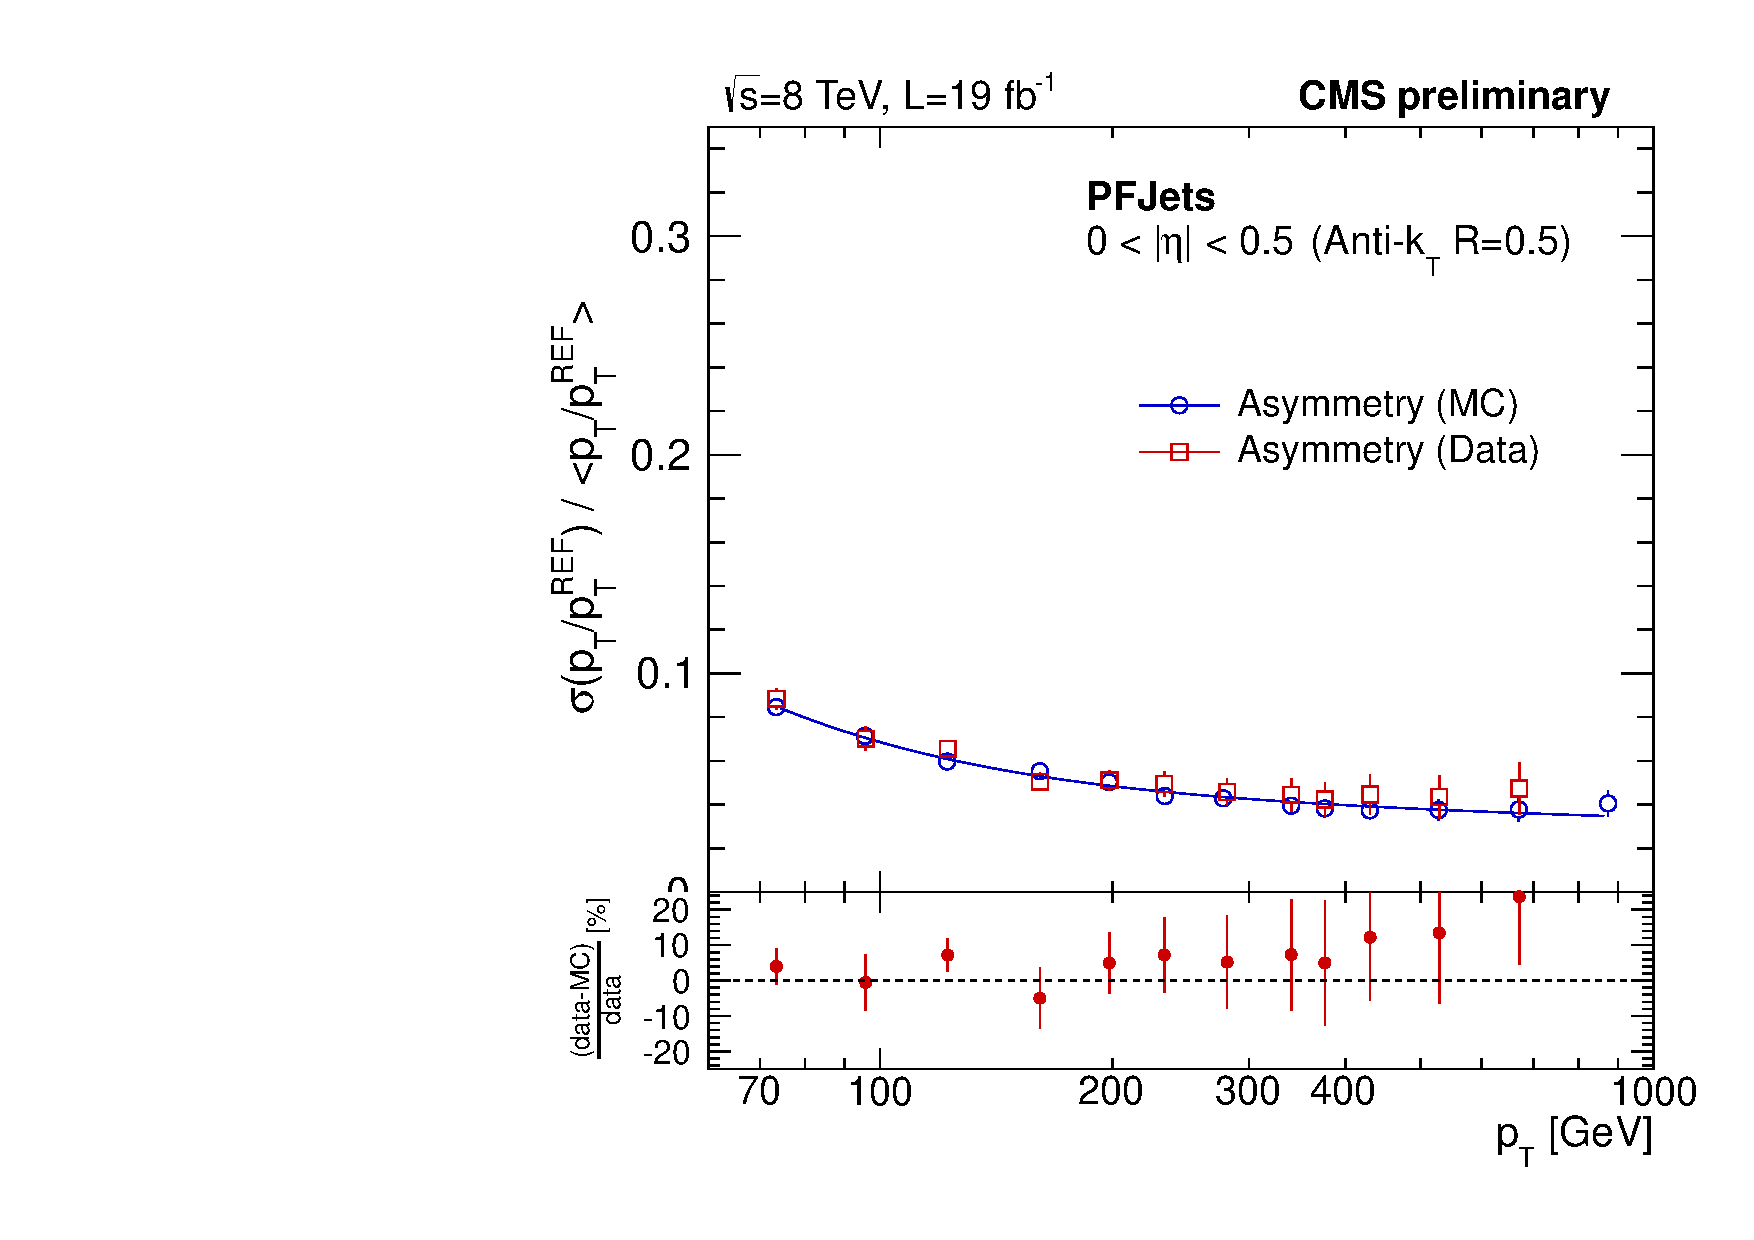
\includegraphics[width=0.45\textwidth,]{figures/ak5pf_relRes}
      \caption{\label{fig:jetRes} The relative $\pt$ resolution as a function of jet $\pt$
              for central jets.}
  \end{center}
\end{figure}

Missing transverse energy (\met) is computed from the same towers of energy deposits 
in the calorimeters that are used for jet-finding; it is the negative of the vectorial
sum of their components transverse to the beam-axis. Corrections are applied to
accommodate the jet energy corrections and the presence of muons~\cite{1748-0221-6-09-P09001}.

